% !TEX TS-program = pdflatex
% academicthesis-luiss-guide.tex
% User and developer guide of the academicthesis class for LUISS Guido
% Carli. Compile from this folder with pdfLaTeX, twice:
%   pdflatex academicthesis-luiss-guide.tex
% Standalone: it does not need the academicthesis class itself.
\documentclass[11pt,a4paper,oneside]{report}
\newcommand{\doctitleshort}{academicthesis --- LUISS guide}
% common/docstyle.tex
% Shared preamble of the academicthesis guides (one guide per university).
% \input it right after \documentclass{report}. A guide sets its accent
% colour afterwards with \colorlet{docaccent}{...}. The guides are
% standalone: they do not need the academicthesis class itself.
\usepackage[T1]{fontenc}
\usepackage[utf8]{inputenc}
\usepackage{lmodern}
\usepackage[english]{babel}
\usepackage[a4paper, margin=2.6cm, headheight=14pt]{geometry}
\usepackage{microtype}
\usepackage{xcolor}
\usepackage{graphicx}
\usepackage{array}
\usepackage{tabularx}
\usepackage{booktabs}
\usepackage{longtable}
\usepackage{listings}
\usepackage{enumitem}
\usepackage{titlesec}
\usepackage{titletoc}
\usepackage{fancyhdr}
\usepackage{tcolorbox}
\tcbuselibrary{skins, breakable}
\usepackage{tikz}
\usetikzlibrary{positioning, arrows.meta}
\usepackage{url}
\usepackage[colorlinks=true, linkcolor=docaccent, urlcolor=docaccent,
            citecolor=docaccent]{hyperref}

% ---- Colours (docaccent is set again by each guide) -------------------
\definecolor{docaccent}{RGB}{31,73,125}
\definecolor{luissblue}{RGB}{21,57,108}      % BlueLuiss, as in the package
\definecolor{bluepoli}{cmyk}{0.4,0.1,0,0.4}  % bluepoli, as in the package
\definecolor{bocconiblue}{RGB}{0,46,93}
\definecolor{docgrey}{gray}{0.45}

% ---- Page and paragraphs ----------------------------------------------
\setlength{\parindent}{0pt}
\setlength{\parskip}{0.55\baselineskip}
\setlength{\emergencystretch}{3em}
\sloppy
\setlist{nosep, topsep=3pt, leftmargin=1.5em}
\renewcommand{\arraystretch}{1.25}
\usepackage{etoolbox}
\AtBeginEnvironment{tabularx}{\small}
\AtBeginEnvironment{longtable}{\small}

% Parts: a full page with a large number and a short description
% \guidepart{<title>}{<one-paragraph introduction>}
\newcommand{\currentpartintro}{}
\titleformat{\part}[display]{\centering\color{docaccent}}
  {\Large\scshape Part \thepart}{10pt}{\Huge\bfseries}
  [\vspace{1.2cm}\begin{minipage}{0.72\linewidth}\centering
   \normalfont\normalsize\color{black}\currentpartintro\end{minipage}]
\newcommand{\guidepart}[2]{\renewcommand{\currentpartintro}{#2}\part{#1}}

\titleformat{\chapter}[display]{\color{docaccent}\normalfont}
  {\large\scshape Chapter \thechapter}{4pt}{\Huge\bfseries}
  [\vspace{2pt}{\color{docaccent}\titlerule[0.8pt]}]
\titlespacing*{\chapter}{0pt}{0pt}{22pt}
\titleformat{\section}{\color{docaccent}\normalfont\Large\bfseries}{\thesection}{0.8em}{}
\titleformat{\subsection}{\color{docaccent}\normalfont\large\bfseries}{\thesubsection}{0.8em}{}
\titleformat{\subsubsection}{\normalfont\normalsize\bfseries}{\thesubsubsection}{0.8em}{}
\titlespacing*{\section}{0pt}{2.4ex plus 1ex}{1ex}
\setcounter{tocdepth}{1}

\pagestyle{fancy}
\fancyhf{}
\fancyhead[L]{\small\color{docgrey}\doctitleshort}
\fancyhead[R]{\small\color{docgrey}\nouppercase{\leftmark}}
\fancyfoot[C]{\small\thepage}
\renewcommand{\headrulewidth}{0.3pt}
\renewcommand{\chaptermark}[1]{\markboth{\thechapter\quad #1}{}}
\fancypagestyle{plain}{\fancyhf{}\renewcommand{\headrulewidth}{0pt}\fancyfoot[C]{\small\thepage}}
\providecommand{\doctitleshort}{academicthesis}

% ---- Names in running text and tables ---------------------------------
\newcommand{\cs}[1]{\texttt{\textbackslash#1}}   % a command
\newcommand{\opt}[1]{\texttt{#1}}                 % an option / key / value
\newcommand{\env}[1]{\texttt{#1}}                 % an environment
\newcommand{\pkg}[1]{\textsf{#1}}                 % a package or class
\DeclareUrlCommand{\file}{\urlstyle{tt}}          % a file name (breaks at - . /)
\renewcommand{\UrlBreaks}{\do\-\do\.\do\/\do\_}
\newcolumntype{Y}{>{\raggedright\arraybackslash}X}
\newcolumntype{L}[1]{>{\raggedright\arraybackslash}p{#1}}
\newcommand{\req}{\textbf{required}}
\newcommand{\optional}{optional}
\newcommand{\na}{\textcolor{docgrey}{---}}

% ---- Code listings -----------------------------------------------------
\lstset{
  basicstyle=\ttfamily\small,
  keywordstyle=\color{docaccent}\bfseries,
  commentstyle=\color{docgrey}\itshape,
  language=[LaTeX]TeX,
  morekeywords={thesissetup, frontpage, luissthesissetup, polimithesissetup,
    bocconithesissetup, major, dedication, frontmatter, mainmatter,
    backmatter, addbibresource, printbibliography, blankpage,
    DeclareThesisBaseClass, DeclareThesisFormats, DeclareThesisSecondPage,
    DeclareThesisOtherLanguages, DeclareThesisClassOption,
    DeclareThesisCoreRequirements, DeclareThesisFrontPage,
    DeclareThesisRequirement, DeclareThesisBibDefaults, ProvideThesisString,
    thesismeta, thesisstring, IfThesisMetaEmptyTF, IfThesisListEmptyTF,
    IfThesisDegreeTF, academicthesislist, AddToHook, ExplSyntaxOn,
    ExplSyntaxOff, ProvidesExplPackage, ProvidesFile, RequirePackage},
  frame=single, rulecolor=\color{docaccent!35},
  backgroundcolor=\color{docaccent!4},
  columns=fullflexible, keepspaces=true, upquote=true,
  breaklines=true, breakatwhitespace=true,
  xleftmargin=4pt, xrightmargin=4pt, aboveskip=8pt, belowskip=8pt,
  literate={à}{{\`a}}1 {è}{{\`e}}1 {é}{{\'e}}1 {ò}{{\`o}}1,
}
\lstdefinestyle{shell}{language={}, keywordstyle={}, commentstyle={}}

% ---- Boxes ---------------------------------------------------------------
% \begin{notebox}[<colour>]{Title} ... \end{notebox}
\newtcolorbox{notebox}[2][docaccent]{enhanced, breakable,
  colback=#1!5, colframe=#1!70, boxrule=0.6pt, arc=2pt,
  left=8pt, right=8pt, top=6pt, bottom=6pt,
  fonttitle=\bfseries\small, coltitle=white, title={#2}}

% A framed page preview: \preview[<width>]{<file>}{<caption>}
\newcommand{\preview}[3][0.42\textwidth]{%
  \begin{minipage}[t]{#1}\centering
    {\setlength{\fboxsep}{0pt}\setlength{\fboxrule}{0.5pt}%
     \fcolorbox{docgrey!50}{white}{\includegraphics[width=\dimexpr\linewidth-1pt\relax]{#2}}}\par
    \vspace{4pt}{\small #3}
  \end{minipage}}

% ---- Title page: \guidetitlepage{<subtitle>}{<figures>} ----------------
\newcommand{\guidetitlepage}[2]{%
  \hypersetup{pageanchor=false}%
  \begin{titlepage}
    \vspace*{2.2cm}
    {\color{docaccent}\rule{\linewidth}{1.2pt}}\par\vspace{14pt}
    {\fontsize{30}{36}\selectfont\bfseries\color{docaccent} academicthesis\par}
    \vspace{10pt}
    {\LARGE #1\par}
    \vspace{6pt}
    {\Large User and developer guide\par}
    \vspace{14pt}
    {\color{docaccent}\rule{\linewidth}{1.2pt}}\par
    \vspace{1.6cm}
    \begin{center}#2\end{center}
    \vfill
    {\large Luca Salvatore\par}
    {\color{docgrey} academicthesis v0.2.0 \quad\textbullet\quad October 2026\par}
  \end{titlepage}%
  \hypersetup{pageanchor=true}}

\graphicspath{{figures/}}

\colorlet{docaccent}{luissblue}

\newcommand{\uniname}{LUISS Guido Carli}
\newcommand{\unishort}{LUISS}
\newcommand{\uniid}{luiss}
\newcommand{\uniotherlangnote}{For correct hyphenation, also list the
  language in the \opt{other-languages} class option, e.g.\
  \opt{other-languages=\{italian\}}; otherwise a warning reminds you.}
\newcommand{\unibibdefault}{for LUISS, author--year: \opt{style=authoryear}}

\hypersetup{pdftitle={academicthesis: LUISS user and developer guide},
            pdfauthor={Luca Salvatore}}

\begin{document}

\guidetitlepage{LUISS Guido Carli}{%
  \preview[0.27\textwidth]{luiss-master-cover}{Bachelor's and master's}\hspace{0.8cm}%
  \preview[0.27\textwidth]{luiss-phd-cover}{PhD}}

{\setlength{\parskip}{0pt}\tableofcontents}

% ######################################################################
\guidepart{User guide}{For students writing a LUISS thesis: what the class does, how to
set it up, every option and command available, and complete examples.}

% ======================================================================
\chapter{What this package does}

Every LUISS thesis opens with the same cover: the university logo, the
degree programme and chair, the title, the names of the supervisor and the
candidate, the academic year. Reproducing it by hand means adjusting
spacing, fonts and alignment, and doing it again when something changes.

\pkg{academicthesis} is a \LaTeX{} class that does this for you. You state
the university and the degree, give the data of the thesis once, and the
class prints the LUISS cover page, the second page with the examination
details and copyright notice, and a consistent layout for the rest of the
thesis:

\begin{lstlisting}
\documentclass[university=luiss, master, language=english]{academicthesis}
\end{lstlisting}

\section{What you get}

\begin{center}
  \preview[0.29\textwidth]{luiss-master-cover}{Bachelor's / master's cover}\hfill
  \preview[0.29\textwidth]{luiss-secondpage}{Second page}\hfill
  \preview[0.29\textwidth]{luiss-phd-cover}{PhD cover}
\end{center}

\begin{itemize}
  \item \textbf{The cover page} for a bachelor's, master's or PhD thesis,
    with the LUISS logo and the title in LUISS blue.
  \item \textbf{The second page}: examination commission (or a statement
    that the thesis has not been defended) and a copyright notice.
  \item \textbf{Front-matter blocks}: abstract, statement of originality,
    acknowledgements and dedication, each in any of the supported
    languages.
  \item \textbf{Labels in your language}: English, Italian or French,
    with singular and plural forms chosen for you (``Supervisor'' or
    ``Supervisors'') and, in Italian, ``Candidato'' or ``Candidata''.
  \item \textbf{Checks}: if a field the cover needs is missing, compilation
    stops with a message naming it, instead of printing a gap.
  \item \textbf{A bibliography} in author--year style, ready to use.
\end{itemize}

\section{How it is organised}

The class has a core shared by every university and one package per
university. For a LUISS thesis the core loads the LUISS package by itself;
you never load it explicitly. Part~\ref{part:dev} of this guide explains
the code for those who want to change it.

% ======================================================================
% common/user-install.tex
% Shared chapter of the user part: installing and compiling.
% Uses \uniname, \unishort, \uniid, set by the guide.
\chapter{Installing and compiling}
\label{ch:install}

\section{Requirements}

\begin{itemize}
  \item A recent \TeX{} distribution: \TeX{}~Live or Mac\TeX{} 2023 or
    later, or an up-to-date MiK\TeX. The class is written in \LaTeX3 and
    needs a modern \LaTeX{} kernel.
  \item \textbf{pdf\LaTeX} is the reference engine, used by all the
    examples in this guide. Xe\LaTeX{} and Lua\LaTeX{} are also accepted
    (the class then loads \pkg{fontspec}).
  \item For the bibliography, \pkg{biblatex} and \pkg{biber}, both part of
    every full \TeX{} distribution. Without them the class falls back to
    \pkg{natbib} and Bib\TeX{} (Section~\ref{sec:bib}).
\end{itemize}

\section{The files you need}

\pkg{academicthesis} is a collection of small packages that load one
another \emph{by name}. For a \unishort{} thesis you need only these:

\begin{tabularx}{\textwidth}{@{}l Y@{}}
\toprule
\textbf{Files} & \textbf{Role} \\
\midrule
\file{core/academicthesis.cls}, \file{core/academicthesis-kernel.sty} & The core class, shared by every university. \\
\file{languages/academicthesis-<language>.ldf} & The words printed on the pages, one file per language (English, Italian, French). \\
\texttt{universities/\uniid/*} & The \unishort{} package: its layout, labels and logos. \\
\bottomrule
\end{tabularx}

The other folders of \file{universities/} belong to other universities and
can be left out.

\section{Three ways to set it up}

\begin{enumerate}
  \item \textbf{Inside the repository.} Copy the \unishort{} showcase in
    \file{showcases/} and keep its first line,
    \begin{lstlisting}
\input{academicthesis-repo-paths}
    \end{lstlisting}
    which tells \LaTeX{} where the package folders are. Then compile with
    any editor, or from a terminal with \texttt{latexmk}.
  \item \textbf{Next to your thesis.} Copy the files listed above into the
    folder of your thesis (without sub-folders) and delete the
    \verb|\input{academicthesis-repo-paths}| line. This is also how to
    use the class on Overleaf: upload the files to the project.
  \item \textbf{Installed in your personal \TeX{} tree}, for example
    \file{~/Library/texmf/tex/latex/academicthesis/} on macOS or
    \file{~/texmf/tex/latex/academicthesis/} on Linux. Every document on the
    computer can then use the class, with no extra line.
\end{enumerate}

\begin{notebox}{Editors}
Texifier/Texpad, TeXShop, TeXstudio, VS Code (LaTeX Workshop) and Overleaf
all work. In Texifier/Texpad, set the typesetter to \emph{TeX Live
(pdfLaTeX)}: its built-in engine is too old for this class.
\end{notebox}

\section{Compiling}

Run pdf\LaTeX{} twice (for the table of contents and cross-references),
with \pkg{biber} between the two runs when the thesis has a bibliography.
\texttt{latexmk} does all of this by itself:

\begin{lstlisting}[style=shell]
latexmk -pdf my-thesis.tex
\end{lstlisting}


% ======================================================================
\chapter{Writing your thesis}
\label{ch:writing}

\section{The shape of a thesis file}

\begin{lstlisting}
\documentclass[university=luiss, master, language=english]{academicthesis}

\usepackage{hyperref}            % your own packages, if any

\thesissetup{                    % the data printed on the cover
  title        = {Title of the Thesis},
  candidate    = {Name Surname},
  idnumber     = {000000},
  degree       = {Economics and Management},
  chair        = {Corporate Finance},
  supervisor   = {Prof. Name Surname},
  academicyear = {2025/2026},
  copyyear     = {2026},
}
\addbibresource{references.bib}

\begin{document}
\frontpage                       % cover page + second page

\frontmatter                     % roman page numbers
\begin{abstractthesis}[keywords = {first, second}]
  The abstract.
\end{abstractthesis}
\tableofcontents

\mainmatter                      % arabic page numbers
\chapter{Introduction}
...
\printbibliography

\backmatter
\begin{acknowledgements}
  Thanks to ...
\end{acknowledgements}
\end{document}
\end{lstlisting}

After \cs{frontpage}, everything is ordinary \LaTeX: chapters, sections,
figures, tables, equations.

\section{Class options}

All options go between the square brackets of \cs{documentclass}.

\begin{tabularx}{\textwidth}{@{}L{3.3cm} L{3.4cm} Y@{}}
\toprule
\textbf{Option} & \textbf{Values} & \textbf{Meaning} \\
\midrule
\opt{university} & \opt{luiss} & Selects the LUISS package. Required. \\
degree & \opt{bachelor}, \opt{master}, \opt{phd} & Written on its own. Chooses the cover. Default: \opt{bachelor}. \\
\opt{language} & \opt{english}, \opt{italian}, \opt{french} & Language of every printed label, and hyphenation. Default: \opt{english}. Short forms: \opt{lang=en}, \opt{lang=it}, \opt{lang=fr}, or just \opt{italian}. \\
\opt{other-languages} & e.g.\ \opt{\{italian,french\}} & Other languages used by single blocks (Section~\ref{sec:blocks}). \\
\opt{no-secondpage} & & Omits the second page (it is printed by default). \\
\opt{discussion} & & The thesis has been defended: the second page shows the date and committee, and \opt{examdate} becomes required. Default: off. \\
\opt{biblatex-options} & e.g.\ \opt{\{style=apa\}} & Options for \pkg{biblatex} (Section~\ref{sec:bib}). \\
anything else & \opt{twoside}, \opt{12pt}, \opt{a4paper}, \dots & Passed to the \pkg{book} class, on which a LUISS thesis is built. \\
\bottomrule
\end{tabularx}

LUISS has a single layout, so the \opt{format} option is not used.

\section{The data of your thesis}
\label{sec:data}

All the data is given with \cs{thesissetup} in the preamble, as
\opt{key = \{value\}} pairs. Write academic titles (``Prof.'', ``Dr.'')
yourself.

\begin{longtable}{@{}L{3.0cm} L{5.1cm} c c@{}}
\toprule
\textbf{Key} & \textbf{Printed as} & \textbf{Bachelor/master} & \textbf{PhD} \\
\midrule
\endhead
\opt{title} & Title, in LUISS blue & \req & \req \\
\opt{subtitle} & Under the title & \optional & \optional \\
\opt{candidate} & ``Candidate'' column & \req & \req \\
\opt{idnumber} & Under the candidate's name & \optional & \optional \\
\opt{gender} & \opt{male}/\opt{female}: ``Candidato'' / ``Candidata'' in Italian & \optional & \optional \\
\opt{degree} & ``Course of \dots'' & \req & \na \\
\opt{chair} & ``Chair of \dots'' & \req & \na \\
\opt{department} & ``Department of \dots'' under the logo & \na & \req \\
\opt{phdtitle} & ``PhD in \dots'' & \na & \req \\
\opt{cycle} & ``Cycle \dots'' & \na & \req \\
\opt{supervisor} / \opt{supervisors} & ``Supervisor(s)'' column & \req & \req \\
\opt{cosupervisor} / \opt{cosupervisors} & ``Co-Supervisor(s)'' column & \optional & \optional \\
\opt{academicyear} & ``Academic Year'' & \req & \req \\
\opt{copyyear} & Second page: ``\textcopyright{} year name'' & recommended & recommended \\
\opt{authoremail}, \opt{website} & Second page: contact lines & \optional & \optional \\
\opt{examdate} & Second page: date of the defence & with \opt{discussion} & with \opt{discussion} \\
\opt{examiners} & Second page: the committee & with \opt{discussion} & with \opt{discussion} \\
\bottomrule
\end{longtable}

\begin{notebox}{Writing the values}
\begin{itemize}
  \item \opt{degree}, \opt{chair}, \opt{department}, \opt{phdtitle} and
    \opt{cycle} are written \emph{without} the words the cover adds:
    \opt{degree = \{Economics and Management\}} prints ``Course of
    Economics and Management''.
  \item \opt{supervisor} takes one name and keeps any comma in it;
    \opt{supervisors} takes several, separated by commas. The label becomes
    ``Supervisors'' by itself. The same holds for \opt{cosupervisor(s)}
    and \opt{examiner(s)}.
  \item \cs{thesissetup} can be used several times; a later value replaces
    an earlier one.
\end{itemize}
\end{notebox}

\section{The major}

A bachelor's or master's thesis may name a major, printed as written
between the course and the chair. It has its own command; either line
works:

\begin{lstlisting}
\major{Major in Corporate Finance}
\luissthesissetup{major = {Major in Corporate Finance}}
\end{lstlisting}

\section{Adjusting the cover: \texorpdfstring{\cs{luissthesissetup}}{\\luissthesissetup}}

\begin{tabularx}{\textwidth}{@{}l l Y@{}}
\toprule
\textbf{Key} & \textbf{Default} & \textbf{Effect} \\
\midrule
\opt{logo-file} & \opt{logoluissblue} & Logo image, file name without extension. The plain \opt{luiss} logo is also shipped. \\
\opt{logo-width} & \opt{0.55\textbackslash textwidth} & Width of the logo. \\
\opt{logo-align} & \opt{left} & \opt{left}, \opt{center} or \opt{right}. \\
\opt{title-align} & \opt{left} & Title and subtitle. \\
\opt{course-align} & \opt{left} & Course and chair (PhD: programme and cycle). \\
\opt{major-align} & \opt{left} & The major. \\
\opt{department-align} & \opt{left} & PhD: the department line. \\
\opt{major} & & The major (above). \\
\bottomrule
\end{tabularx}

All alignment keys except \opt{logo-align} also accept \opt{l}, \opt{c},
\opt{r}. For example, a centred cover:

\begin{lstlisting}
\luissthesissetup{logo-align = center, title-align = center,
                  course-align = center, major-align = center}
\end{lstlisting}

\section{The second page}

\cs{frontpage} prints the second page after the cover, unless the class
option \opt{no-secondpage} is given.

\begin{itemize}
  \item \textbf{Top}: without \opt{discussion}, ``The present thesis has
    not been defended.''; with \opt{discussion}, the defence date
    (\opt{examdate}) and the committee (\opt{examiners}).
  \item \textbf{Bottom}: the title, ``\textcopyright{} \opt{copyyear}
    \opt{candidate}'', a reservation of rights, the author, and the e-mail
    and website when given.
\end{itemize}

Give \opt{copyyear}, or the notice will have no year.

% ======================================================================
\chapter{Front matter and bibliography}

% common/user-blocks.tex
% Shared sections of the user part: front-matter blocks and bibliography.
% Uses \unishort, \uniotherlangnote and \unibibdefault, set by the guide.
\section{Abstract, originality, acknowledgements, dedication}
\label{sec:blocks}

The core class provides four front-matter blocks. They are written the
same way at every university; the \unishort{} package only sets their look.

\begin{tabularx}{\textwidth}{@{}l l Y@{}}
\toprule
\textbf{Block} & \textbf{Options} & \textbf{Default heading (English)} \\
\midrule
\cs{begin}\opt{\{abstractthesis\}} & \opt{language}, \opt{keywords}, \opt{title} & Abstract \\
\cs{begin}\opt{\{originality\}} & \opt{language}, \opt{title} & Statement of Originality \\
\cs{begin}\opt{\{acknowledgements\}} & \opt{language}, \opt{title} & Acknowledgments \\
\cs{dedication}\opt{[...]\{text\}} & \opt{language} & none: the text alone on its page \\
\bottomrule
\end{tabularx}

\begin{itemize}
  \item \opt{language=} writes the block in another language: its heading,
    the ``Keywords'' label and the hyphenation follow that language.
    Without it, the block uses the main language of the thesis.
    \uniotherlangnote
  \item \opt{keywords=} prints a list of keywords after the abstract.
  \item \opt{title=} replaces the default heading.
\end{itemize}

Abstracts, statements of originality and acknowledgements are listed in
the table of contents. An English abstract followed by an Italian one:

\begin{lstlisting}
\begin{abstractthesis}[keywords = {corporate finance, valuation}]
  The English abstract.
\end{abstractthesis}
\begin{abstractthesis}[language = italian,
                       keywords = {finanza aziendale, valutazione}]
  L'abstract in italiano.
\end{abstractthesis}
\dedication{To my family.}
\end{lstlisting}

\section{Bibliography}
\label{sec:bib}

The class loads \pkg{biblatex} with \pkg{biber} for you; do not load
\pkg{biblatex} again in your preamble. Its style is, in order of priority:
the options you give with the class option \opt{biblatex-options}; the
university's default (\unibibdefault); otherwise a numeric style.

\begin{lstlisting}
\documentclass[..., biblatex-options={style=apa}]{academicthesis}
\addbibresource{references.bib}   % in the preamble
...
\printbibliography                % where the bibliography goes
\end{lstlisting}

If \pkg{biblatex} is not installed, the class warns and uses \pkg{natbib}
with Bib\TeX{} behind the same two commands, so the thesis still compiles.


% ======================================================================
\chapter{Complete examples}

\section{Bachelor's or master's thesis}

\begin{lstlisting}
\documentclass[university=luiss, master, language=english, twoside,
               discussion, other-languages={italian}]{academicthesis}

\major{Major in Corporate Finance}

\thesissetup{
  title        = {Title of the Thesis},
  subtitle     = {An Optional Subtitle},
  candidate    = {Name Surname},
  idnumber     = {000000},
  degree       = {Economics and Management},
  chair        = {Corporate Finance},
  supervisor   = {Prof. Name Surname},
  cosupervisor = {Prof. Name Surname},
  academicyear = {2025/2026},
  copyyear     = {2026},
  authoremail  = {name.surname@example.com},
  examdate     = {12 July 2026},              % because of `discussion'
  examiners    = {Prof. A, Prof. B, Prof. C},
}
\addbibresource{references.bib}

\begin{document}
\frontpage

\frontmatter
\begin{abstractthesis}[keywords = {first, second}]
  The abstract.
\end{abstractthesis}
\begin{abstractthesis}[language = italian, keywords = {primo, secondo}]
  Il sommario in italiano.
\end{abstractthesis}
\dedication{To my family.}
\tableofcontents

\mainmatter
\chapter{Introduction}
...
\printbibliography

\backmatter
\begin{acknowledgements}
  Thanks to ...
\end{acknowledgements}
\end{document}
\end{lstlisting}

For a bachelor's thesis write \opt{bachelor}. Without \opt{discussion},
leave out \opt{examdate} and \opt{examiners}.

\section{PhD thesis}

\begin{lstlisting}
\documentclass[university=luiss, phd, language=english, twoside]{academicthesis}

\thesissetup{
  title        = {Title of the Dissertation},
  candidate    = {Name Surname},
  idnumber     = {000000},
  department   = {Economics and Finance},   % "Department of ..."
  phdtitle     = {Economics},               % "PhD in ..."
  cycle        = {XXXVIII},                 % "Cycle ..."
  supervisors  = {Prof. Name Surname},
  academicyear = {2025/2026},
  copyyear     = {2026},
}

\begin{document}
\frontpage
\frontmatter
\begin{abstractthesis}
  The abstract.
\end{abstractthesis}
\tableofcontents
\mainmatter
\chapter{Introduction}
...
\end{document}
\end{lstlisting}

Complete, compilable versions are in \file{showcases/example-luiss-bachelor.tex}
and \file{showcases/example-luiss-phd.tex}.

% ======================================================================
\chapter{Troubleshooting}

\begin{longtable}{@{}L{5.2cm} L{4.2cm} L{4.6cm}@{}}
\toprule
\textbf{Message (abridged)} & \textbf{Cause} & \textbf{Fix} \\
\midrule
\endhead
Missing required thesis metadata: `\textit{key}' & A required field is not in \cs{thesissetup} & Add it; the message shows an example. See Section~\ref{sec:data}. \\
Missing required thesis metadata: `examdate' & \opt{discussion} without the defence date & Add \opt{examdate}, or remove \opt{discussion}. \\
Missing required thesis metadata: `chair' & Bachelor's or master's thesis without the chair & Add \opt{chair}. \\
Missing required thesis metadata: `cycle' (or `department', `phdtitle') & PhD data missing & Add it to \cs{thesissetup}. \\
University `luiss' does not offer formats & A \opt{format} option & Remove it. \\
File `academicthesis.cls' not found & \LaTeX{} cannot see the class files & Keep the line that inputs \file{academicthesis-repo-paths}, or copy the files next to the thesis (Chapter~\ref{ch:install}). \\
File `logoluissblue' not found & Logo file missing & Copy the files of \file{universities/luiss/} too. \\
Warning: `french' \dots{} was not loaded by babel & A block with \opt{language=french} & Add \opt{french} to the \opt{other-languages} option. \\
Warning: biblatex is not available & \pkg{biblatex} not installed & Install it, or keep the \pkg{natbib} fallback. \\
\bottomrule
\end{longtable}

\section*{Quick reference}

\begin{lstlisting}
\documentclass[university=luiss, bachelor|master|phd,
               language=english|italian|french, other-languages={...},
               no-secondpage, discussion, biblatex-options={...}]{academicthesis}
\luissthesissetup{major={...}, logo-file=..., logo-width=...,
                  logo-align=left|center|right, title-align=...,
                  course-align=..., major-align=..., department-align=...}
\thesissetup{title, subtitle, candidate, idnumber, gender,
             degree, chair,                 % bachelor/master
             department, phdtitle, cycle,   % PhD
             supervisor(s), cosupervisor(s), academicyear,
             copyyear, authoremail, website, examdate, examiners}
\frontpage
\begin{abstractthesis}[language=..., keywords=..., title=...]
  ... \end{abstractthesis}
\begin{originality}[language=..., title=...] ... \end{originality}
\begin{acknowledgements}[language=..., title=...]
  ... \end{acknowledgements}
\dedication[language=...]{...}
\end{lstlisting}

% ######################################################################
\guidepart{Developer guide}{For those who maintain or extend the code: first how the shared
core works, then how the LUISS package is built on it.}
\label{part:dev}

% common/dev-core.tex
% Shared chapter of the developer part: how the core works.
% Uses \unishort and \uniid, set by the guide.
\chapter{How the core works}
\label{ch:core}

This chapter describes the part of the code that every university shares.
The next chapter builds on it to explain the \unishort{} package. The
reader is assumed to know \LaTeXe{} package writing; \LaTeX3 (\pkg{expl3})
names are explained where they matter.

\section{Design principles}

\begin{description}[leftmargin=0pt, labelindent=0pt, itemsep=4pt]
  \item[The core knows no university.] \file{academicthesis.cls} never
    mentions LUISS, Politecnico di Milano or Bocconi. A university package
    plugs into a small number of \emph{registries} (front pages, required
    fields, bibliography defaults) and \emph{declarations} (base class,
    formats, second page, extra languages, extra class options) that the
    core consults at the right moment.
  \item[A university knows only the core.] A university package uses the
    kernel's public commands and never another university's code, so each
    one can be versioned, shipped and installed on its own.
  \item[Files are found by name, never by folder.] Every \cs{LoadClass},
    \cs{RequirePackage}, \cs{input} and \cs{includegraphics} names a file,
    not a path. Once installed in a \TeX{} tree, kpathsea finds each file
    whatever package shipped it; in the repository, the search path is
    extended instead of changing the code (Section~\ref{sec:searchpath}).
  \item[One data store, one vocabulary.] All thesis data lives in a single
    property list with the same key names at every university. Universities
    change \emph{wording} through string files, not key names.
  \item[Logic in \LaTeX3, typesetting in \LaTeXe.] Option handling,
    registries and validation are written in \pkg{expl3}; everything that
    puts text on the page is written in ordinary \LaTeX{} syntax, where
    spaces and blank lines behave as usual (Section~\ref{sec:catcodes}).
\end{description}

\section{Files}

\begin{tabularx}{\textwidth}{@{}l Y@{}}
\toprule
\textbf{File} & \textbf{Role} \\
\midrule
\file{core/academicthesis.cls} & The class: options, base class, fonts and languages, bibliography, loading the university, labels, \cs{frontpage}, second page, front-matter blocks, page styles, validation. \\
\file{core/academicthesis-kernel.sty} & The shared API: messages, metadata store, \cs{thesissetup}, lists, registries, early-configuration commands, university loader, string store. Loaded first, by the class. \\
\file{languages/academicthesis-<lang>.ldf} & Generic strings for one language (\cs{ProvideThesisString} calls only). \\
\file{universities/<uni>/academicthesis-<uni>.cfg} & Early configuration, read \emph{before} the base class is loaded. \\
\file{universities/<uni>/academicthesis-<uni>.sty} & The university package proper. \\
\file{universities/<uni>/academicthesis-<uni>-*.def} & Layout code in normal \LaTeX{} syntax, read by the \file{.sty}. \\
\file{universities/<uni>/academicthesis-<uni>-<lang>.ldf} & Optional: the university's wording of core strings, and its own strings. \\
\file{showcases/academicthesis-repo-paths.tex} & Lets the examples find the repository folders (not part of any package). \\
\bottomrule
\end{tabularx}

\section{What happens when a thesis is compiled}
\label{sec:sequence}

\begin{center}
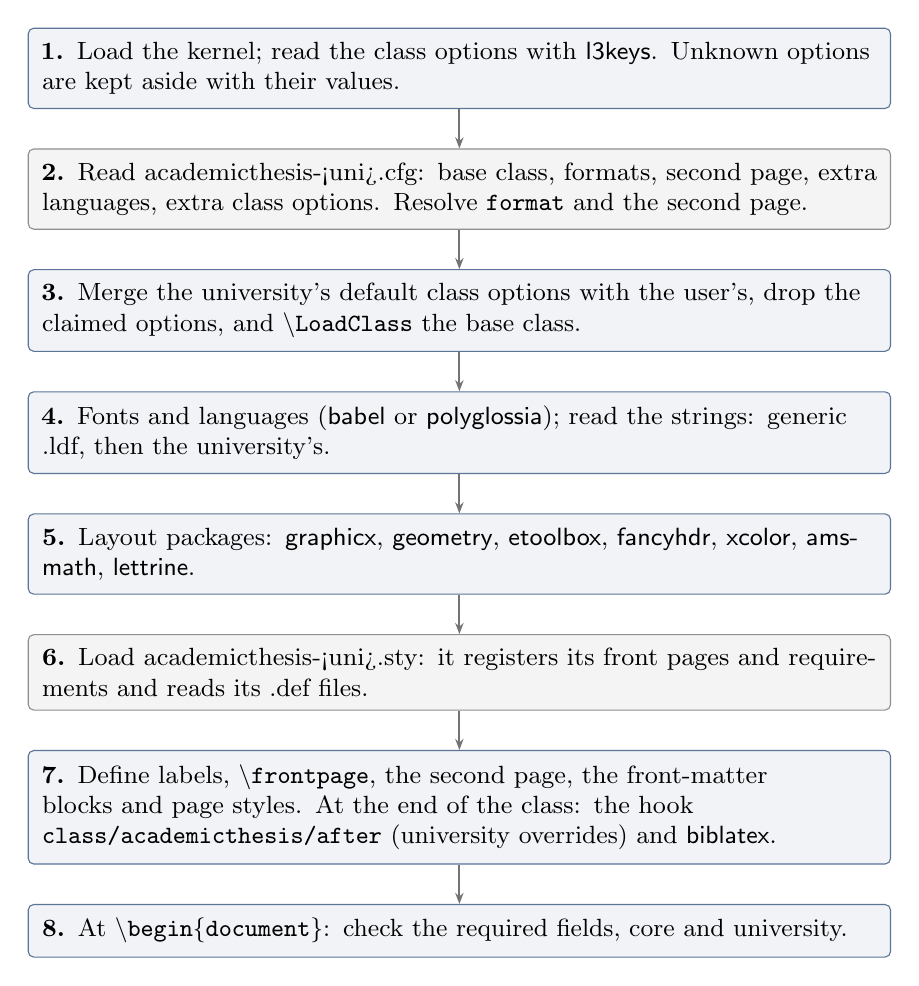
\begin{tikzpicture}[node distance=5mm,
    stepbox/.style={draw=docaccent!70, fill=docaccent!6, rounded corners=2pt,
      text width=10.6cm, align=left, font=\small, inner sep=5pt},
    unibox/.style={stepbox, draw=docgrey!80, fill=docgrey!8},
    arr/.style={-{Stealth[length=4pt]}, draw=docgrey, thick}]
  \node[stepbox] (s1) {\textbf{1.} Load the kernel; read the class options with \pkg{l3keys}. Unknown options are kept aside with their values.};
  \node[unibox, below=of s1] (s2) {\textbf{2.} Read \file{academicthesis-<uni>.cfg}: base class, formats, second page, extra languages, extra class options. Resolve \opt{format} and the second page.};
  \node[stepbox, below=of s2] (s3) {\textbf{3.} Merge the university's default class options with the user's, drop the claimed options, and \cs{LoadClass} the base class.};
  \node[stepbox, below=of s3] (s4) {\textbf{4.} Fonts and languages (\pkg{babel} or \pkg{polyglossia}); read the strings: generic \file{.ldf}, then the university's.};
  \node[stepbox, below=of s4] (s5) {\textbf{5.} Layout packages: \pkg{graphicx}, \pkg{geometry}, \pkg{etoolbox}, \pkg{fancyhdr}, \pkg{xcolor}, \pkg{amsmath}, \pkg{lettrine}.};
  \node[unibox, below=of s5] (s6) {\textbf{6.} Load \file{academicthesis-<uni>.sty}: it registers its front pages and requirements and reads its \file{.def} files.};
  \node[stepbox, below=of s6] (s7) {\textbf{7.} Define labels, \cs{frontpage}, the second page, the front-matter blocks and page styles. At the end of the class: the hook \opt{class/academicthesis/after} (university overrides) and \pkg{biblatex}.};
  \node[stepbox, below=of s7] (s8) {\textbf{8.} At \cs{begin}\opt{\{document\}}: check the required fields, core and university.};
  \foreach \a/\b in {s1/s2,s2/s3,s3/s4,s4/s5,s5/s6,s6/s7,s7/s8} \draw[arr] (\a) -- (\b);
\end{tikzpicture}
\end{center}

Grey steps are where the university's own files run. Two consequences
matter when writing a university package:

\begin{itemize}
  \item The \file{.cfg} runs before \cs{LoadClass}: it may only use the
    early-configuration commands (Section~\ref{sec:cfg}) and \pkg{expl3}
    logic, not packages or document commands.
  \item The \file{.sty} runs \emph{before} the core defines its labels,
    blocks and page styles (step~7). To change one of those, a university
    wraps its redefinition in the hook that \LaTeX{} runs once the class
    has finished:
\begin{lstlisting}
\AddToHook{class/academicthesis/after}{%
  \RenewDocumentCommand\thesiskeywords{mm}{...}}
\end{lstlisting}
\end{itemize}

\section{The early configuration file}
\label{sec:cfg}

\file{academicthesis-<uni>.cfg} is read with \pkg{expl3} syntax on (spaces
are ignored; write \verb|~| for a space). Its commands concern only the
active university, so they take no university argument.

\begin{longtable}{@{}L{5.8cm} L{8.6cm}@{}}
\toprule
\textbf{Command} & \textbf{Meaning} \\
\midrule
\endhead
\cs{DeclareThesisBaseClass}\newline\opt{\{<class>\}\{<options>\}} & Base class (\pkg{book}, \pkg{article}, \dots) and its default options. A default is dropped when the user chose another option of the same group: \opt{11pt} beats a default \opt{12pt}, \opt{oneside} beats \opt{twoside}. Default: \pkg{book} with no options. \\
\cs{DeclareThesisFormats}\newline\opt{\{<list>\}\{<default>\}} & The values accepted by \opt{format=}. Resolved at once, so the rest of the file can branch on \cs{g\_\_academicthesis\_format\_tl}. A university that declares none rejects \opt{format=}. \\
\cs{DeclareThesisSecondPage}\newline\opt{\{true|false\}} & Default for the second page (examination commission and copyright). The user can override it with \opt{secondpage} / \opt{no-secondpage}. Default: \opt{true}. \\
\cs{DeclareThesisOtherLanguages}\newline\opt{\{<list>\}} & Languages always loaded with \pkg{babel}, besides the main one. \\
\cs{DeclareThesisClassOption}\newline\opt{\{<name>\}\{<default>\}} & Claims a \cs{documentclass} option for the university; it is no longer passed to the base class. \opt{name} alone means \opt{true}. Read it with \cs{academicthesis\_class\_option:n}\opt{\{<name>\}} or, in normal syntax, \cs{thesisclassoption}\opt{\{<name>\}}. \\
\cs{DeclareThesisCoreRequirements}\newline\opt{\{true|false\}} & Whether the core checks its own required fields (title, candidate, academic year, degree, supervisors). The university's requirements are checked either way. Default: \opt{true}. \\
\bottomrule
\end{longtable}

\section{Thesis data}

\subsection{The store}

All data given with \cs{thesissetup} goes into one global property list.
\cs{thesissetup} is a thin \pkg{l3keys} front-end: each key writes one
entry.

\begin{tabularx}{\textwidth}{@{}L{6.2cm} Y@{}}
\toprule
\textbf{\pkg{expl3} (in \file{.sty}/\file{.cfg})} & \textbf{Effect} \\
\midrule
\cs{academicthesis\_meta\_set:nn}\newline\opt{\{key\}\{value\}} & Store a value. \\
\cs{academicthesis\_meta\_get:n}\newline\opt{\{key\}} & The value (expandable; empty when missing). \\
\cs{academicthesis\_meta\_if\_empty:nTF} & Test for an empty or missing value (also \opt{p}, \opt{T}, \opt{F}). \\
\cs{academicthesis\_list\_set:nn}, \cs{\_set\_csv:nn}, \cs{\_add:nn} & Set a list to one item, to comma-separated items, or append one. \\
\cs{academicthesis\_list\_count:n}, \cs{academicthesis\_list\_if\_empty:nTF} & Number of items; emptiness test. \\
\bottomrule
\end{tabularx}

\begin{tabularx}{\textwidth}{@{}L{6.2cm} Y@{}}
\toprule
\textbf{Normal syntax (in \file{.def})} & \textbf{Effect} \\
\midrule
\cs{thesismeta}\newline\opt{\{key\}} & The value (expandable). \\
\cs{IfThesisMetaEmptyTF}\newline\opt{\{key\}\{empty\}\{not empty\}} & Branch on a value. \\
\cs{academicthesislist}\newline\opt{[sep]\{list\}} & Typeset a list; default separator \verb|\\|. \\
\cs{thesislistcount}\newline\opt{\{list\}}, \cs{IfThesisListEmptyTF} & Count items; branch on emptiness. \\
\cs{IfThesisDegreeTF}\newline\opt{\{bachelor|master|phd\}\{yes\}\{no\}} & Branch on the degree. \\
\cs{thesisclassoption}\newline\opt{\{name\}} & Value of a claimed class option. \\
\bottomrule
\end{tabularx}

The standard keys are \opt{title}, \opt{subtitle}, \opt{candidate},
\opt{idnumber}, \opt{degree}, \opt{chair}, \opt{department}, \opt{major},
\opt{phdtitle}, \opt{cycle}, \opt{academicyear}, \opt{copyyear},
\opt{examdate}, \opt{authoremail}, \opt{website}, \opt{dedication},
\opt{abstract}, \opt{keywords}, \opt{coordinator} and \opt{gender}, plus the
lists \opt{supervisors}, \opt{cosupervisors}, \opt{examiners} and
\opt{tutors} (each with a singular key that sets one item without
splitting at commas). A university may store keys of its own with
\cs{academicthesis\_meta\_set:nn}; the core never reads them.

\subsection{Validation}

At \cs{begin}\opt{\{document\}} the core checks its own fields (unless
switched off in the \file{.cfg}) and then every entry registered with

\begin{lstlisting}
\DeclareThesisRequirement{<uni>}{<boolean>}{<key>}{<example>}
\end{lstlisting}

whose university is the active one and whose \pkg{expl3} boolean is true:
\cs{c\_true\_bool} (always), \cs{g\_\_academicthesis\_bachelor\_bool},
\cs{\_master\_bool} or \cs{\_phd\_bool}. A missing field raises the error
\emph{Missing required thesis metadata: `<key>'}, whose help text shows
\opt{<example>}.

\section{Registries}

\begin{tabularx}{\textwidth}{@{}L{6.2cm} Y@{}}
\toprule
\textbf{Command} & \textbf{Meaning} \\
\midrule
\cs{DeclareThesisFrontPage}\newline\opt{\{<uni>\}\{<degree>\}\{<cs>\}} & \cs{frontpage} looks up \opt{<uni>.<degree>} and runs \opt{<cs>}; if nothing is registered, it raises \emph{No front page registered}. The command typesets its own page(s). \\
\cs{DeclareThesisRequirement}\newline\opt{\{<uni>\}\{<bool>\}\{<key>\}\{<ex>\}} & A required field (above). \\
\cs{DeclareThesisBibDefaults}\newline\opt{\{<uni>\}\{<options>\}} & \pkg{biblatex} options used when the user gives no \opt{biblatex-options}. \\
\bottomrule
\end{tabularx}

\section{Strings and languages}

Every printed word comes from a string store, one per language, filled by
\cs{ProvideThesisString}\opt{\{<key>\}\{<text>\}}. For each language the
kernel reads \file{academicthesis-<lang>.ldf} and then, if it exists,
\file{academicthesis-<uni>-<lang>.ldf}. A university file reuses the core
keys to change the wording (for instance \opt{SupervisorLabel}) and may add
keys of its own.

\cs{thesisstring}\opt{\{<key>\}} prints a string in the language currently
selected for strings: the main language, or the one a block switched to
with \opt{language=}. It falls back to the main language, then to the key
name, so a missing translation never stops compilation.

The labels \cs{authorlabel}, \cs{supervisorlabel} and \cs{cosupervisorlabel}
choose the singular or plural string from the length of the list, and the
female form of the candidate label from \opt{gender}.

\section{Front matter, second page, page styles}

\begin{itemize}
  \item \cs{frontpage} dispatches to the registered front page, then
    prints the second page if it is on.
  \item \env{abstractthesis}, \env{originality}, \env{acknowledgements}
    and \cs{dedication} all go through one option parser (\opt{language},
    \opt{title}, \opt{keywords}). Headings use \cs{thesisfrontchapter},
    which writes \cs{chapter*} or \cs{section*} depending on whether the
    base class has chapters, and adds the table-of-contents entry.
  \item Universities can restyle without touching the parser:
    \cs{thesiskeywords}\opt{\{<label>\}\{<keywords>\}} prints the keywords;
    \cs{thesisacknowledgementsbegin}\opt{\{<heading>\}} and
    \cs{thesisacknowledgementsend} frame the acknowledgements.
  \item The core defines the page styles \opt{Thesis}, \opt{acknowledgments}
    and \opt{plain}; \cs{frontmatter} switches to \opt{plain} and
    \cs{mainmatter} to \opt{Thesis}. Under a base class without chapters,
    the core supplies light versions of \cs{frontmatter}, \cs{mainmatter}
    and \cs{backmatter}.
\end{itemize}

\section{Two rules for writing layout code}
\label{sec:catcodes}

\paragraph{Typeset in normal syntax.} Under \cs{ExplSyntaxOn} spaces are
ignored and blank lines do not end paragraphs, which silently breaks any
text. University packages therefore keep their \pkg{expl3} code in the
\file{.sty} and put pages in \file{.def} files read with the document
catcodes:

\begin{lstlisting}
\cs_new_protected:Npn \__myuni_input_layout:n #1
  {
    \cctab_begin:N \c_document_cctab   % no group: definitions survive
      \file_input:n { academicthesis-myuni-#1.def }
    \cctab_end:
  }
\end{lstlisting}

\paragraph{Never load a package from a \texttt{.def} file.} When a package
loaded from there ends, \LaTeX{} restores the syntax of the class that is
loading everything, \pkg{expl3}, and every space that follows is lost. The
\file{.sty} loads the packages before reading the \file{.def}.

\section{Search path in the repository}
\label{sec:searchpath}

Inside the repository the files sit in sub-folders, which \TeX{} does not
search. Two mechanisms make them visible without any path in the code:

\begin{itemize}
  \item \textbf{latexmk}: the root \file{latexmkrc} adds \file{core//},
    \file{languages//} and \file{universities//} to \opt{TEXINPUTS} (the
    trailing \opt{//} also searches sub-folders).
  \item \textbf{Any editor}: \file{showcases/academicthesis-repo-paths.tex},
    input before \cs{documentclass}, extends \LaTeX's \cs{input@path} with
    the folders. \cs{input@path} does not search sub-folders, so it lists
    each university folder; a new university needs a line there.
\end{itemize}

\section{Messages}

All messages use the \pkg{expl3} message module \opt{academicthesis}, so
they read \emph{Class academicthesis Error} and carry a help text.

\begin{tabularx}{\textwidth}{@{}l Y@{}}
\toprule
\textbf{Name} & \textbf{When} \\
\midrule
\opt{missing-metadata} & A required field is empty. \\
\opt{missing-frontpage} & No front page registered for the university and degree. \\
\opt{unknown-university} & No \file{academicthesis-<uni>.sty} found. \\
\opt{missing-config} & The \file{.sty} exists but the \file{.cfg} does not. \\
\opt{unknown-format}, \opt{no-formats} & A \opt{format} the university does not declare, or any \opt{format} at a university with none. \\
\opt{missing-language} & No \file{.ldf} for the chosen language (falls back to English). \\
\opt{bibliography-fallback} & \pkg{biblatex} unavailable (warning). \\
\bottomrule
\end{tabularx}

A university defines its own messages in the same module with
\cs{msg\_new:nnnn}\opt{\{academicthesis\}\{<uni>-<name>\}\{...\}\{...\}}.

\section{Adding a university, in short}

\begin{enumerate}
  \item Create \file{universities/<uni>/} with
    \file{academicthesis-<uni>.cfg} (at least \cs{DeclareThesisBaseClass}).
  \item Write \file{academicthesis-<uni>.sty}: \cs{RequirePackage}
    \opt{\{academicthesis-kernel\}}, setup keys, packages, requirements,
    then read the \file{.def} files.
  \item In each \file{.def}, define the front page and register it with
    \cs{DeclareThesisFrontPage} for each degree offered.
  \item Add \file{academicthesis-<uni>-<lang>.ldf} files for its wording.
  \item Add its folder to \file{showcases/academicthesis-repo-paths.tex}
    and a showcase.
\end{enumerate}

Nothing in \file{core/}, \file{languages/} or another university changes.


% ======================================================================
\chapter{The LUISS package}
\label{ch:unidev}

\section{Files}

\begin{tabularx}{\textwidth}{@{}l Y@{}}
\toprule
\textbf{File} & \textbf{Role} \\
\midrule
\file{academicthesis-luiss.cfg} & Base class \pkg{book} with no default options; second page on. \\
\file{academicthesis-luiss.sty} & Setup keys, cover building blocks (\pkg{expl3}), loading of the cover file, requirements, bibliography defaults. \\
\file{academicthesis-luiss-bachelor-master.def} & The bachelor's and master's cover, in normal syntax. \\
\file{academicthesis-luiss-phd.def} & The PhD cover, in normal syntax. \\
\file{logoluissblue.pdf}, \file{luiss.pdf} & Logos. \\
\bottomrule
\end{tabularx}

LUISS has no \file{academicthesis-luiss-<lang>.ldf}: its labels are the
core ones (``Supervisor'', ``Candidate'', ``Course of'', ``Chair of'',
``PhD in'', ``Cycle'', ``Department of'').

\section{The early configuration}

\begin{lstlisting}
\DeclareThesisBaseClass { book } { }
\DeclareThesisSecondPage { true }
\end{lstlisting}

No formats, no extra class options, the core requirements on: the user
chooses paper size and sides freely.

\section{The package, section by section}

\paragraph{1. LUISS metadata.} \opt{major} is stored under the private key
\opt{luiss-major} through the key family
\opt{academicthesis-luiss/meta}, used by \cs{major}. The core never reads
it. (The core's own \opt{major} key exists for other universities; the
LUISS cover reads \opt{luiss-major}.)

\paragraph{2. Layout controller.} \cs{luissthesissetup} sets the key family
\opt{academicthesis-luiss/layout}: \opt{logo-file}, \opt{logo-width} and
the five alignment keys. Each alignment is stored in a token list
(\cs{l\_\_luiss\_title\_align\_tl} and so on) and normalised to \opt{l},
\opt{c} or \opt{r} by \cs{\_\_luiss\_norm\_align:N} after every call. The
old name \cs{LuissThesisController} is kept as an alias.

\paragraph{3. Building blocks.} The cover is assembled from blocks written
in \pkg{expl3}, each reading the metadata store:

\begin{tabularx}{\textwidth}{@{}l Y@{}}
\toprule
\textbf{Block (document-level name)} & \textbf{Prints} \\
\midrule
\cs{luiss@logobox} & The logo, at the chosen width and alignment. \\
\cs{luiss@departmentline} & ``Department of \opt{department}'' (PhD). \\
\cs{luiss@programmeblock}\opt{\{first\}\{middle\}\{second\}} & The course or programme line, an optional middle line, a gap and the chair or cycle line. \\
\cs{luiss@majorline} & The major, when given. \\
\cs{luiss@titleblock} & Title in \opt{BlueLuiss} (RGB 21,57,108) and subtitle. \\
\cs{luiss@namesblock} & Supervisor(s), co-supervisor(s) and candidate with ID, in labelled columns; two layouts depending on whether there are co-supervisors. \\
\cs{luiss@academicyear} & ``Academic Year'' and the year, centred. \\
\bottomrule
\end{tabularx}

Fonts come from the core: \cs{TitleFont}, \cs{SubtitleFont},
\cs{LowerFont}. The colour \opt{BlueLuiss} is also used for drop caps
(\cs{LettrineFontHook}).

\paragraph{4. Loading the cover.} The \file{.sty} reads exactly one
\file{.def} with the document catcodes: \file{-phd.def} when the degree is
\opt{phd}, \file{-bachelor-master.def} otherwise.

\paragraph{5. Requirements.}

\begin{lstlisting}
% bachelor and master: degree and chair
\DeclareThesisRequirement { luiss } \g__academicthesis_bachelor_bool { degree } {...}
\DeclareThesisRequirement { luiss } \g__academicthesis_master_bool   { degree } {...}
\DeclareThesisRequirement { luiss } \g__academicthesis_bachelor_bool { chair }  {...}
\DeclareThesisRequirement { luiss } \g__academicthesis_master_bool   { chair }  {...}
% PhD: cycle, department, programme
\DeclareThesisRequirement { luiss } \g__academicthesis_phd_bool { cycle }      {...}
\DeclareThesisRequirement { luiss } \g__academicthesis_phd_bool { department } {...}
\DeclareThesisRequirement { luiss } \g__academicthesis_phd_bool { phdtitle }   {...}
\end{lstlisting}

The core adds title, candidate, academic year, supervisors, the degree for
bachelor and master, and \opt{examdate} with \opt{discussion}.

\paragraph{6. Bibliography.} Author--year by default:
\begin{lstlisting}
\DeclareThesisBibDefaults { luiss } { style = authoryear, backend = biber }
\end{lstlisting}

\section{The cover files}

Both \file{.def} files follow the same plan and differ only in what they
pass to the blocks:

\begin{lstlisting}
\newcommand\luiss@frontpage@bachelormaster{%
  \begin{titlepage}%
    \thispagestyle{empty}%
    \newgeometry{left=2.75cm, right=2.75cm, top=3cm, bottom=2.5cm}%
    \luiss@logobox\par
    \vspace{0.1\textheight}%
    \luiss@programmeblock
      {\thesisstring{CourseOf} \thesismeta{degree}}%
      {\luiss@majorline}%
      {\thesisstring{ChairOf} \thesismeta{chair}}%
    \par\vfill
    \luiss@titleblock\par\vfill
    \luiss@namesblock\par
    \vspace{0.1\textheight}%
    \luiss@academicyear\par
    \vspace*{0.05\textheight}%
    \restoregeometry
  \end{titlepage}}
\DeclareThesisFrontPage{luiss}{bachelor}{\luiss@frontpage@bachelormaster}
\DeclareThesisFrontPage{luiss}{master}{\luiss@frontpage@bachelormaster}
\end{lstlisting}

The PhD page adds \cs{luiss@departmentline} under the logo and passes
``PhD in \opt{phdtitle}'' and ``Cycle \opt{cycle}'' to the programme
block. The second page is the core's, not the package's.

\section{Common changes}

\begin{tabularx}{\textwidth}{@{}L{5cm} Y@{}}
\toprule
\textbf{To change\dots} & \textbf{Edit\dots} \\
\midrule
the order or spacing of the cover & the \file{.def} of that degree. \\
how a block looks (columns, colour, rule) & the block in section~3 of the \file{.sty}. \\
a label's wording & add \file{academicthesis-luiss-<lang>.ldf} with \cs{ProvideThesisString} for the core key (e.g.\ \opt{SupervisorLabel}). \\
which fields are required & section~5 of the \file{.sty}. \\
the default bibliography & section~6 of the \file{.sty}. \\
the default class options & the \file{.cfg}. \\
\bottomrule
\end{tabularx}

Keep the two rules of Section~\ref{sec:catcodes}: text in the \file{.def}
files, packages loaded only from the \file{.sty}.

% ======================================================================
\chapter*{Licence and credits}
\addcontentsline{toc}{chapter}{Licence and credits}

\pkg{academicthesis} is released under the \LaTeX{} Project Public Licence
(LPPL) 1.3c or later; copyright 2025--2026 Luca Salvatore. The LUISS name
and logo belong to LUISS Guido Carli. \pkg{academicthesis} is not
published by LUISS: before submitting a thesis, check the current rules of
your degree programme.

\end{document}
